\documentclass{article}
\usepackage{ctex}
\usepackage{geometry}
\geometry{a4paper, scale=0.8}
\usepackage{graphicx}
\usepackage{subfigure}
\usepackage{float}
\usepackage{enumitem}
\usepackage{amsmath}
\usepackage{amssymb}
\usepackage{makecell}

\title{HW04}
\author{PB19071405\ 王昊元}
\date{2022 年 06 月 12 日}

\begin{document}
    \maketitle

    \section*{第1题}
    系统用例图如下:
    \begin{figure}[H]
        \centering
        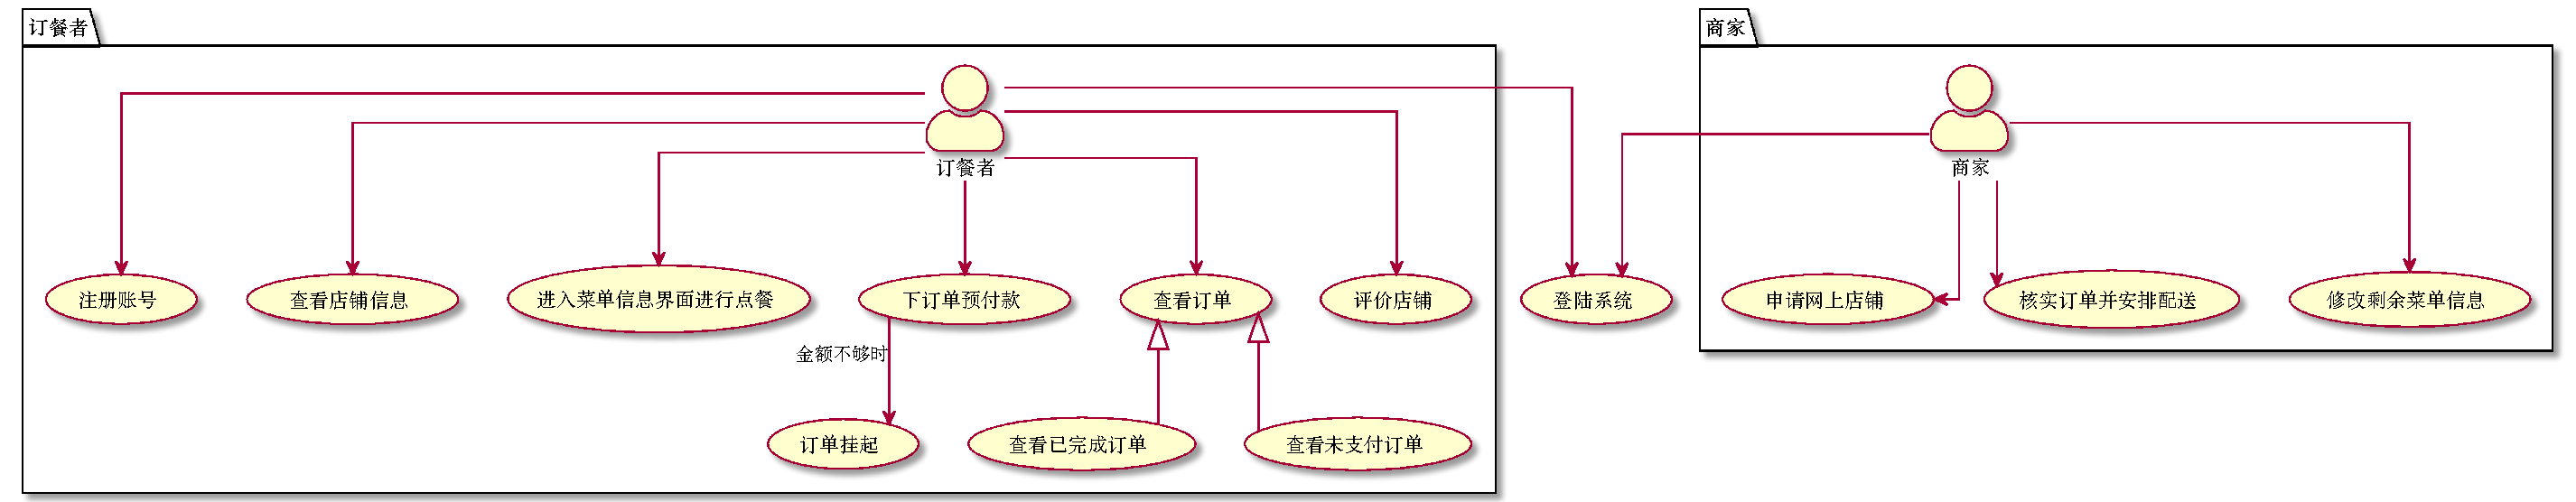
\includegraphics[width=\textwidth]{./fig/hw04/1.pdf}
        \caption{网上订餐系统用例图}
    \end{figure}
    订餐的用例说明如下:
    \begin{table}[H]
        \centering
        \caption{用例1说明}
        \begin{tabular}{cm{12cm}}
            \hline
            用例编号 & 1 \\
            \hline
            用例名称 & 注册账号 \\
            \hline
            参与者 & 订餐者 \\
            \hline
            用例描述 & 订餐者需要注册一个账号用于系统登录 \\
            \hline
            前置条件 & 无 \\
            \hline
            触发条件 & 参与者发起注册/点击注册按钮 \\
            \hline
            正常流程 & 用户进入注册界面; 用户输入用户名和密码,并重复输入一次密码; 用户提交注册信息; 系统检查信息合理性; 系统保存用户信息; 注册完成 \\
            \hline
            异常流程 & 账户名与已有账户重复、密码不符合要求、两次密码输入不一致:返回注册界面 \\
            \hline
            后置条件 & 用户的账号密码信息保存到系统数据库,系统进入登陆界面 \\
            \hline
        \end{tabular}
    \end{table}
    \begin{table}[H]
        \centering
        \caption{用例2说明}
        \begin{tabular}{cm{12cm}}
            \hline
            用例编号 & 2 \\
            \hline
            用例名称 & 登陆系统 \\
            \hline
            参与者 & 订餐者、商家 \\
            \hline
            用例描述 & 订餐者和商家需要登陆系统完成相应的订餐操作 \\
            \hline
            前置条件 & 订餐者需要已注册账号,商家需要已申请网上店铺 \\
            \hline
            触发条件 & 参与者登陆系统/点击登录按钮 \\
            \hline
            正常流程 & 用户进入登陆界面; 用户输入用户名和密码; 用户提交登陆信息; 系统检查信息合理性; 登陆完成 \\
            \hline
            异常流程 & 账户名不存在、密码与用户名不符:返回登陆界面 \\
            \hline
            后置条件 & 用户登陆成功,进入相应界面(订餐者进入店铺选择页面,商家进入店铺详情页面/后台) \\
            \hline
        \end{tabular}
    \end{table}
    \begin{table}[H]
        \centering
        \caption{用例3说明}
        \begin{tabular}{cm{12cm}}
            \hline
            用例编号 & 3 \\
            \hline
            用例名称 & 查看店铺信息 \\
            \hline
            参与者 & 订餐者 \\
            \hline
            用例描述 & 订餐者登陆系统后可以查看店铺信息 \\
            \hline
            前置条件 & 参与者需要已经登陆系统 \\
            \hline
            触发条件 & 参与者点击店铺入口 \\
            \hline
            正常流程 & 用户浏览店铺列表; 用户选择一个店铺点击进入; 用户跳转到店铺详情页面; 用户查看菜单信息 \\
            \hline
            异常流程 & 店铺不存在:返回店铺列表界面 \\
            \hline
            后置条件 & 订餐者进入店铺详情页面,查看店铺信息 \\
            \hline
        \end{tabular}
    \end{table}
    \begin{table}[H]
        \centering
        \caption{用例4说明}
        \begin{tabular}{cm{12cm}}
            \hline
            用例编号 & 4 \\
            \hline
            用例名称 & 进入菜单信息界面进行点餐 \\
            \hline
            参与者 & 订餐者 \\
            \hline
            用例描述 & 订餐者在一家店铺的菜单信息界面点餐 \\
            \hline
            前置条件 & 订餐者已经查看店铺信息 \\
            \hline
            触发条件 & 订餐者点击点餐按钮 \\
            \hline
            正常流程 & 用户进入菜单信息界面; 用户选择菜品; 用户将已选菜品加入购物车 \\
            \hline
            异常流程 & 菜品不存在、商品选择数量超过库存(菜品售罄为一种特殊情况):提示用户 \\
            \hline
            后置条件 & 订餐者完整菜品选择 \\
            \hline
        \end{tabular}
    \end{table}
    \begin{table}[H]
        \centering
        \caption{用例5说明}
        \begin{tabular}{cm{12cm}}
            \hline
            用例编号 & 5 \\
            \hline
            用例名称 & 下订单预付款 \\
            \hline
            参与者 & 订餐者 \\
            \hline
            用例描述 & 订餐者为订餐下单并准备付款 \\
            \hline
            前置条件 & 订餐者已经完成菜品选择 \\
            \hline
            触发条件 & 订餐者点击下单按钮 \\
            \hline
            正常流程 & 用户进入结算界面; 用户确认订单; 用户选择支付方式; 进入支付界面; 完成支付; 下单成功 \\
            \hline
            异常流程 & 付款失败、订单超时、取消订单:返回菜品选择页面;金额不足:订单挂起 \\
            \hline
            后置条件 & 订餐者完成订单支付,系统提示商家,系统记录交易信息 \\
            \hline
        \end{tabular}
    \end{table}
    \begin{table}[H]
        \centering
        \caption{用例6说明}
        \begin{tabular}{cm{12cm}}
            \hline
            用例编号 & 6 \\
            \hline
            用例名称 & 查看订单 \\
            \hline
            参与者 & 订餐者 \\
            \hline
            用例描述 & 订餐者查看历史订单 \\
            \hline
            前置条件 & 订单者已登陆系统 \\
            \hline
            触发条件 & 订餐者点击查看订单按钮 \\
            \hline
            正常流程 & 用户进入订单信息界面; 用户选择特定订单并查看订单详细信息 \\
            \hline
            异常流程 & 无 \\
            \hline
            后置条件 & 无 \\
            \hline
        \end{tabular}
    \end{table}
    \begin{table}[H]
        \centering
        \caption{用例7说明}
        \begin{tabular}{cm{12cm}}
            \hline
            用例编号 & 7 \\
            \hline
            用例名称 & 评价店铺 \\
            \hline
            参与者 & 订餐者 \\
            \hline
            用例描述 & 订餐者在订单完成后可以对店铺进行评价 \\
            \hline
            前置条件 & 订餐者完成下单付款并完成用餐 \\
            \hline
            触发条件 & 订餐者点击店铺评价按钮 \\
            \hline
            正常流程 & 用户进入评价界面; 用户填写并提交评价信息; 评价完成 \\
            \hline
            异常流程 & 点评符合字数要求:提示用户修改 \\
            \hline
            后置条件 & 系统记录评价信息并提示店家 \\
            \hline
        \end{tabular}
    \end{table}
    \begin{table}[H]
        \centering
        \caption{用例8说明}
        \begin{tabular}{cm{12cm}}
            \hline
            用例编号 & 8 \\
            \hline
            用例名称 & 申请网上店铺 \\
            \hline
            参与者 & 商家 \\
            \hline
            用例描述 & 商家在系统上申请店铺以营业 \\
            \hline
            前置条件 & 无 \\
            \hline
            触发条件 & 商家点击申请店铺按钮 \\
            \hline
            正常流程 & 用户进入申请界面; 用户提供所需信息并提交申请信息; 系统检测信息合理性;系统记录申请信息 \\
            \hline
            异常流程 & 所提供信息不满足相应要求:提示用户修改 \\
            \hline
            后置条件 & 系统记录申请信息,系统提示审核人员进行审核 \\
            \hline
        \end{tabular}
    \end{table}
    \begin{table}[H]
        \centering
        \caption{用例9说明}
        \begin{tabular}{cm{12cm}}
            \hline
            用例编号 & 9 \\
            \hline
            用例名称 & 核实订单并安排配送 \\
            \hline
            参与者 & 商家 \\
            \hline
            用例描述 & 商家核实系统上的订单信息并安排配送 \\
            \hline
            前置条件 & 订单者完成下单/系统记录订单信息 \\
            \hline
            触发条件 & 系统提示商家订单信息/提示商家新订单 \\
            \hline
            正常流程 & 商家进入订单详情页面;商家查看订单信息,核实后确认;系统根据信息安排外卖员,并将信息发给外卖员;商家将餐品交给外卖员;外卖员接单后到店取餐;外卖员配送餐品至订餐者;配送完成 \\
            \hline
            异常流程 & 订餐者取消订单:提示商家; 没有匹配外卖员/外卖员无法到达:提示商家和订餐者并启动赔偿 \\
            \hline
            后置条件 & 无 \\
            \hline
        \end{tabular}
    \end{table}
    \begin{table}[H]
        \centering
        \caption{用例10说明}
        \begin{tabular}{cm{12cm}}
            \hline
            用例编号 & 10 \\
            \hline
            用例名称 & 修改剩余菜单信息 \\
            \hline
            参与者 & 商家 \\
            \hline
            用例描述 & 商家修改菜单的信息 \\
            \hline
            前置条件 & 商家申请店铺成功 \\
            \hline
            触发条件 & 商家点击编辑按钮 \\
            \hline
            正常流程 & 商家进入编辑页面; 修改商品信息(上架/下架/修改/预售等); 完成编辑并保存; 系统记录商品信息 \\
            \hline
            异常流程 & 超时:提示用户 \\
            \hline
            后置条件 & 系统记录新商品信息并更新店铺信息 \\
            \hline
        \end{tabular}
    \end{table}
    \section*{第2题}
    系统用例图如下:
    \begin{figure}[H]
        \centering
        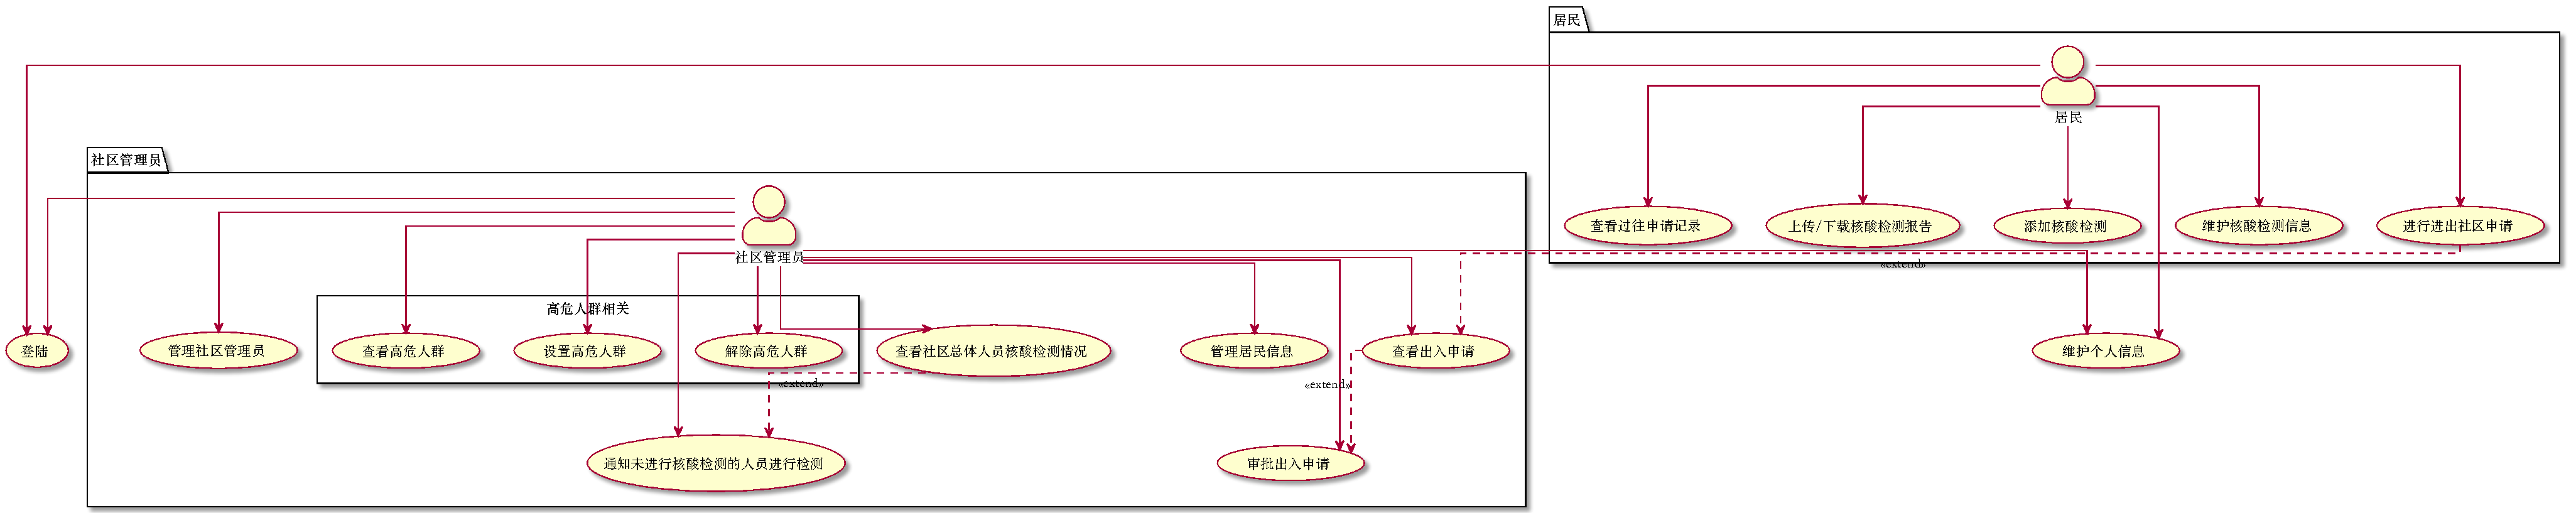
\includegraphics[width=\textwidth]{./fig/hw04/2.1.pdf}
        \caption{社区核酸检测管理系统用例图}
    \end{figure}
    居民申请进出社区的泳道活动图如下:
    \begin{figure}[H]
        \centering
        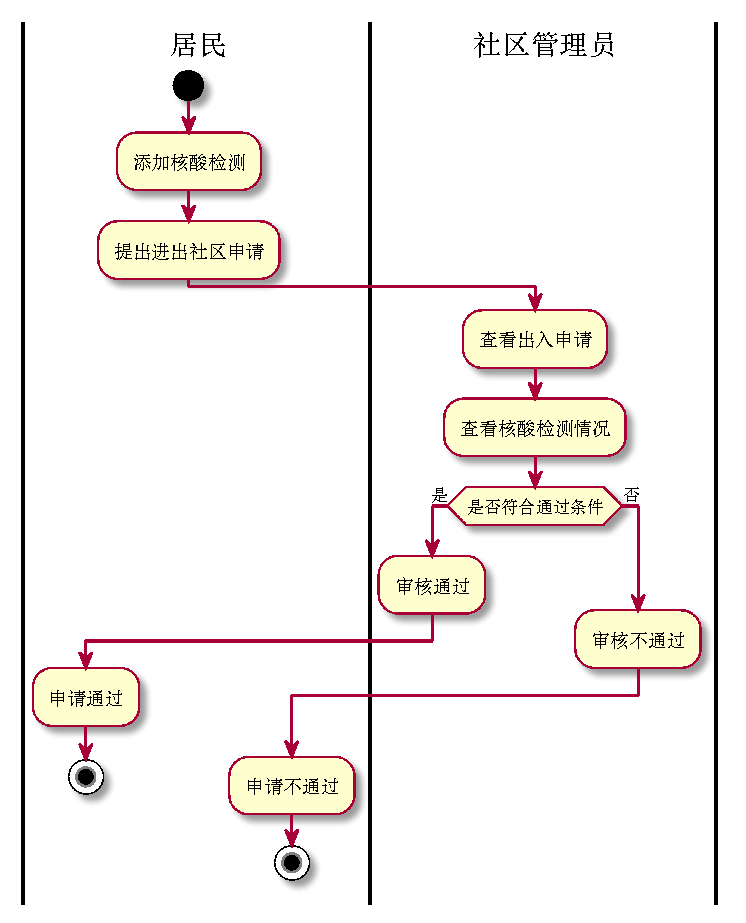
\includegraphics[width=0.8\textwidth]{./fig/hw04/2.2.pdf}
        \caption{居民申请进出社区的泳道活动图}
    \end{figure}
\end{document}